\documentclass[aspectratio=169, 10pt]{beamer}

% --- Theme & Styling ---
\usetheme{Madrid}
\usecolortheme{seahorse}

\definecolor{googleblue}{RGB}{26, 115, 232}
\definecolor{googlered}{RGB}{234, 67, 53}
\definecolor{googleyellow}{RGB}{251, 188, 4}
\definecolor{googlegreen}{RGB}{52, 168, 83}
\definecolor{darknavy}{RGB}{15, 23, 42}
\definecolor{codebg}{RGB}{241, 245, 249}

\setbeamercolor{palette primary}{bg=darknavy,fg=white}
\setbeamercolor{palette secondary}{bg=googleblue,fg=white}
\setbeamercolor{palette tertiary}{bg=darknavy,fg=white}
\setbeamercolor{titlelike}{bg=darknavy,fg=white}
\setbeamercolor{structure}{fg=googleblue}
\setbeamercolor{block title}{bg=googleblue,fg=white}
\setbeamercolor{block body}{bg=codebg,fg=black}

\setbeamertemplate{navigation symbols}{}
\setbeamertemplate{footline}[frame number]

% --- Packages ---
\usepackage{amsmath, amssymb, amsfonts}
\usepackage{graphicx}
\usepackage{tikz}
\usetikzlibrary{shapes.geometric, arrows.meta, positioning, calc, chains, matrix, backgrounds}
\usepackage{listings}
\usepackage{booktabs}
\usepackage{multicol}
\usepackage{array}

% --- Code Listing Syntax ---
\lstset{
    backgroundcolor=\color{codebg},
    basicstyle=\ttfamily\scriptsize,
    breaklines=true,
    captionpos=b,
    commentstyle=\color{googlegreen},
    keywordstyle=\color{googleblue}\bfseries,
    stringstyle=\color{googlered},
    numbers=left,
    numberstyle=\tiny\color{gray},
    frame=single,
    rulecolor=\color{gray!30}
}

% --- Title Information ---
\title[Tesseract-BP Architecture]{Tesseract-BP: High-Performance Belief Propagation \& Layered Serial SIMD Vectorization}
\subtitle{The Tiered QEC Decoding Vision \& High-Throughput Min-Sum Architecture}
\author[Tesseract Team]{Tesseract QEC Decoding Team}
\institute[Google DeepMind]{Advanced Agentic Coding / Quantum Decoding Group}
\date{\today}

\begin{document}

% --- Title Slide ---
\begin{frame}
    \titlepage
\end{frame}

% --- Table of Contents ---
\begin{frame}{Lecture Overview}
    \tableofcontents
\end{frame}

% --- Include Sections ---
\section{The Tesseract Vision \& QEC Decoding Fundamentals}

\begin{frame}{The Grand Vision: Tesseract as a One-Stop QEC Engine}
    \begin{block}{Repository Objective}
        Make \textbf{Tesseract} the unified, highly optimized \textbf{one-stop platform for all offline Quantum Error Correction (QEC) decoding needs}.
    \end{block}
    
    \vspace{0.3cm}
    \begin{columns}[T]
        \begin{column}{0.31\textwidth}
            \centering
            \colorbox{googleblue!15}{\parbox{0.92\textwidth}{
                \textbf{\textcolor{googleblue}{Tier 1: Fast Baseline}}\\[0.1cm]
                \textbf{Belief Propagation (BP) + OSD}\\[0.1cm]
                \scriptsize Fast heuristic evaluation ($10^5-10^6$ shots/s). First stop for code construction \& rapid feedback.
            }}
        \end{column}
        
        \begin{column}{0.31\textwidth}
            \centering
            \colorbox{googleyellow!20}{\parbox{0.92\textwidth}{
                \textbf{\textcolor{darknavy}{Tier 2: Refined Accuracy}}\\[0.1cm]
                \textbf{MultiPass / Gari Tesseract}\\[0.1cm]
                \scriptsize Heuristic path-search refinement for near-threshold verification.
            }}
        \end{column}
        
        \begin{column}{0.31\textwidth}
            \centering
            \colorbox{googlegreen!15}{\parbox{0.92\textwidth}{
                \textbf{\textcolor{googlegreen}{Tier 3: Exact Optimum}}\\[0.1cm]
                \textbf{Full Tesseract (A* Search)}\\[0.1cm]
                \scriptsize Exact optimal path decoding for ground-truth physical error rate bounds.
            }}
        \end{column}
    \end{columns}
\end{frame}

\begin{frame}{Recommended Code Development Workflow}
    \centering
    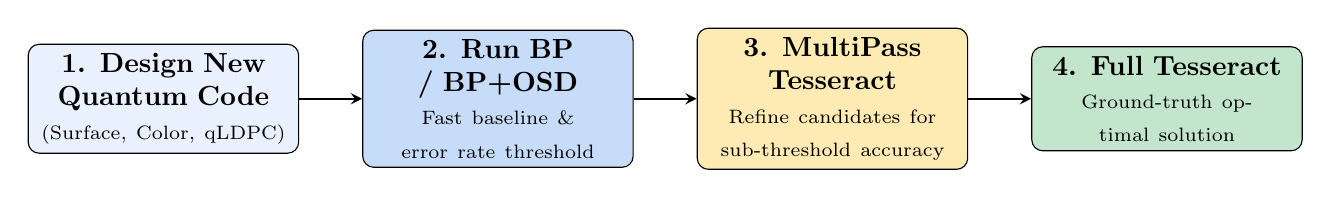
\begin{tikzpicture}[node distance=1.5cm, auto, >=stealth]
        \node [rectangle, draw, fill=googleblue!10, rounded corners, text width=3.2cm, align=center, minimum height=1cm] (code) {\textbf{1. Design New Quantum Code}\\\scriptsize (Surface, Color, qLDPC)};
        \node [rectangle, draw, fill=googleblue!25, rounded corners, text width=3.2cm, align=center, minimum height=1cm, right=0.8cm of code] (bp) {\textbf{2. Run BP / BP+OSD}\\\scriptsize Fast baseline \& error rate threshold};
        \node [rectangle, draw, fill=googleyellow!30, rounded corners, text width=3.2cm, align=center, minimum height=1cm, right=0.8cm of bp] (multipass) {\textbf{3. MultiPass Tesseract}\\\scriptsize Refine candidates for sub-threshold accuracy};
        \node [rectangle, draw, fill=googlegreen!30, rounded corners, text width=3.2cm, align=center, minimum height=1cm, right=0.8cm of multipass] (full) {\textbf{4. Full Tesseract}\\\scriptsize Ground-truth optimal solution};
        
        \draw [->, thick] (code) -- (bp);
        \draw [->, thick] (bp) -- (multipass);
        \draw [->, thick] (multipass) -- (full);
    \end{tikzpicture}
    
    \vspace{0.5cm}
    \begin{block}{Why start with BP?}
        \begin{itemize}
            \item Ultra-high throughput enables sampling millions of Monte Carlo shots in seconds.
            \item Direct measurement of syndrome graph connectivity and trapping set vulnerabilities.
        \end{itemize}
    \end{block}
\end{frame}

\begin{frame}{Quantum Error Correction \& Syndrome Decoding}
    \begin{columns}[T]
        \begin{column}{0.5\textwidth}
            \begin{block}{Physical Error to Syndrome Mapping}
                \begin{itemize}
                    \item Physical errors $e \in \mathbb{F}_2^N$ occur on physical qubits.
                    \item Quantum non-demolition (QND) stabilizer measurements yield syndrome $s \in \mathbb{F}_2^M$:
                          $$s = H \cdot e \pmod 2$$
                    \item \textbf{Parity-Check Matrix ($H$)}: $M \times N$ binary matrix mapping $N$ potential error channels to $M$ detectors.
                \end{itemize}
            \end{block}
        \end{column}
        
        \begin{column}{0.48\textwidth}
            \begin{block}{The Decoding Problem}
                Given observed syndrome $s$, find the most likely error candidate $\hat{e}$ satisfying:
                $$H \cdot \hat{e} = s \pmod 2$$
                \begin{itemize}
                    \item \textbf{Maximum Likelihood Decoding (MLD)}:
                          $$\hat{e}_{MLD} = \arg\max_{e: He=s} P(e)$$
                    \item \textbf{NP-Hardness}: MLD over arbitrary linear block codes is strictly NP-hard!
                \end{itemize}
            \end{block}
        \end{column}
    \end{columns}
\end{frame}

\begin{frame}{Syndrome Generation from Stim DEM}
    \begin{block}{Detector Error Model (DEM)}
        \begin{itemize}
            \item Stim describes circuit-level noise (T1/T2, gate faults) as probabilistic error mechanisms.
            \item Each error mechanism flips a specific set of parity check measurements (detectors).
        \end{itemize}
    \end{block}
    
    \begin{block}{Constructing the Parity Check Matrix ($H$)}
        \begin{itemize}
            \item \textbf{Columns ($N$)}: Correspond to independent error mechanisms in the DEM.
            \item \textbf{Rows ($M$)}: Correspond to detectors (syndrome bits) triggered by errors.
            \item $H_{i,j} = 1$ if error $j$ triggers detector $i$, otherwise $0$.
            \item \textbf{Priors}: Each column $j$ has a prior probability $p_j$ defined by the DEM.
        \end{itemize}
    \end{block}
\end{frame}

\begin{frame}{The Shift to qLDPC Codes \& Tanner Graphs}
    \begin{columns}[T]
        \begin{column}{0.55\textwidth}
            \begin{block}{Quantum Low-Density Parity-Check (qLDPC)}
                \begin{itemize}
                    \item Standard Surface Codes scale as $O(d^2)$ physical qubits per logical qubit.
                    \item \textbf{qLDPC Codes} (e.g., Bivariate Bicycle Codes $[[72,12,6]]$, $[[144,12,12]]$) achieve constant encoding rate:
                          $$\frac{K}{N} = \text{const} > 0$$
                    \item Parity-check matrix $H$ is sparse (constant row/column weights).
                \end{itemize}
            \end{block}
        \end{column}
        
        \begin{column}{0.42\textwidth}
            \begin{block}{Bipartite Tanner Graph}
                \centering
                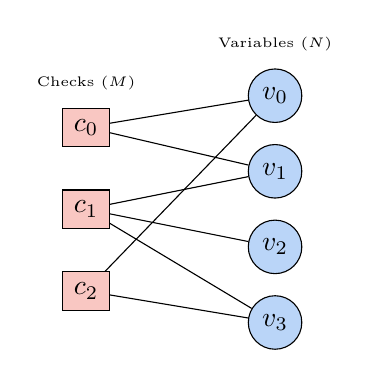
\begin{tikzpicture}[scale=0.8, >=stealth]
                    % Check nodes
                    \node[draw, rectangle, fill=googlered!30, inner sep=4pt] (c0) at (0, 2.5) {$c_0$};
                    \node[draw, rectangle, fill=googlered!30, inner sep=4pt] (c1) at (0, 1.2) {$c_1$};
                    \node[draw, rectangle, fill=googlered!30, inner sep=4pt] (c2) at (0, -0.1) {$c_2$};
                    
                    % Variable nodes
                    \node[draw, circle, fill=googleblue!30, inner sep=3pt] (v0) at (3, 3) {$v_0$};
                    \node[draw, circle, fill=googleblue!30, inner sep=3pt] (v1) at (3, 1.8) {$v_1$};
                    \node[draw, circle, fill=googleblue!30, inner sep=3pt] (v2) at (3, 0.6) {$v_2$};
                    \node[draw, circle, fill=googleblue!30, inner sep=3pt] (v3) at (3, -0.6) {$v_3$};
                    
                    % Edges
                    \draw (c0) -- (v0); \draw (c0) -- (v1);
                    \draw (c1) -- (v1); \draw (c1) -- (v2); \draw (c1) -- (v3);
                    \draw (c2) -- (v0); \draw (c2) -- (v3);
                    
                    \node[above=0.1cm of c0] {\tiny Checks ($M$)};
                    \node[above=0.1cm of v0] {\tiny Variables ($N$)};
                \end{tikzpicture}
            \end{block}
        \end{column}
    \end{columns}
\end{frame}

\section{qLDPC Codes \& Belief Propagation Foundations}

\begin{frame}{Brief History of Belief Propagation}
    \begin{itemize}
        \item \textbf{1962 — Robert Gallager}: Introduces Low-Density Parity-Check (LDPC) codes and iterative belief propagation decoding in his MIT PhD thesis. (Ignored for decades due to hardware limitations!).
        \item \textbf{1982 — Judea Pearl}: Formalizes Belief Propagation on Bayesian networks and Directed Acyclic Graphs (DAGs).
        \item \textbf{1996 — David MacKay \& Radford Neal}: Rediscover LDPC codes and demonstrate near Shannon-limit capacity performance over noisy channels.
        \item \textbf{2000s-Present — Quantum Adaptation}: Adaptation of BP and Min-Sum message-passing algorithms to Quantum LDPC and surface codes for real-time and offline decoding.
    \end{itemize}
\end{frame}

\begin{frame}{Log-Likelihood Ratio (LLR) Mathematics}
    \begin{block}{LLR Definition}
        For a binary random variable $v_i \in \{0, 1\}$, the Log-Likelihood Ratio is defined as:
        $$L(v_i) = \ln \left( \frac{P(v_i = 0)}{P(v_i = 1)} \right)$$
        \begin{itemize}
            \item $L(v_i) > 0 \implies v_i = 0$ is more likely (no error).
            \item $L(v_i) < 0 \implies v_i = 1$ is more likely (error present).
            \item $|L(v_i)|$ represents the \textbf{reliability} / confidence of the belief.
        \end{itemize}
    \end{block}
    
    \begin{block}{Channel Prior Initialization from Stim DEM}
        Given physical error probability $p_i$ from the Stim Detector Error Model:
        $$L_{\text{prior}}(v_i) = \ln \left( \frac{1 - p_i}{p_i} \right)$$
        For integer SIMD execution, LLRs are scaled and fixed into 32-bit signed integers (\texttt{LLR\_INT}).
    \end{block}
\end{frame}

\begin{frame}{Sum-Product vs. Min-Sum Update Rules}
    \begin{block}{Sum-Product Check Update (Exact)}
        Check-to-variable message $R_{c \rightarrow v}$ in exact Sum-Product:
        $$\tanh\left(\frac{R_{c \rightarrow v}}{2}\right) = \left( \prod_{v' \in N(c) \setminus \{v\}} \text{sign}(Q_{v' \rightarrow c}) \right) \times \prod_{v' \in N(c) \setminus \{v\}} \tanh\left(\frac{|Q_{v' \rightarrow c}|}{2}\right)$$
        \textit{Requires expensive transcendental evaluations ($\tanh, \text{atanh}$) per edge per iteration!}
    \end{block}
    
    \begin{block}{Min-Sum Approximation (Fast Vectorizable)}
        Applies the identity $\tanh(x) \approx \min(x)$ for large LLRs:
        $$R_{c \rightarrow v} = \alpha \times \left( \prod_{v' \in N(c) \setminus \{v\}} \text{sign}(Q_{v' \rightarrow c}) \right) \times \min_{v' \in N(c) \setminus \{v\}} |Q_{v' \rightarrow c}|$$
        \begin{itemize}
            \item \textbf{Normalization / Damping Factor}: $\alpha = 0.625$ compensates for Min-Sum over-estimation.
            \item Purely dynamic comparison and integer addition $\rightarrow$ ideal for SIMD hardware execution!
        \end{itemize}
    \end{block}
\end{frame}

\begin{frame}{BP Scheduling Modalities: Parallel vs. Serial}
    \begin{columns}[T]
        \begin{column}{0.48\textwidth}
            \begin{block}{1. Synchronous (Parallel) Schedule}
                Two distinct phases per iteration:
                \begin{enumerate}
                    \item Compute all $V \rightarrow C$ messages concurrently.
                    \item Compute all $C \rightarrow V$ messages concurrently.
                \end{enumerate}
                \textbf{Pros}: Massive potential parallelism.\\
                \textbf{Cons}: Delayed message propagation; requires 2x memory iteration state.
            \end{block}
        \end{column}
        
        \begin{column}{0.48\textwidth}
            \begin{block}{2. Asynchronous (Serial) Schedule}
                Sequential update across nodes:
                \begin{enumerate}
                    \item Select node (variable or check).
                    \item Immediately update posterior belief $L_v$.
                    \item Immediately propagate updated belief to neighboring nodes.
                \end{enumerate}
                \textbf{Pros}: 2x faster iteration convergence!\\
                \textbf{Cons}: Requires careful ordering to prevent L1 cache thrashing.
            \end{block}
        \end{column}
    \end{columns}
\end{frame}

\begin{frame}{LDPC Trapping Sets \& Convergence Obstacles}
    \begin{columns}[T]
        \begin{column}{0.55\textwidth}
            \begin{block}{What is an LDPC Trapping Set?}
                \begin{itemize}
                    \item A sub-graph of variable nodes and check nodes that fails to converge due to symmetric graph loops.
                    \item In QEC codes (Color codes, Bivariate Bicycle codes), short 4-cycles and 6-cycles form \textbf{symmetric trapping sets}.
                    \item Under fixed linear serial schedules ($0 \rightarrow N-1$), beliefs bounce back and forth between states endlessly.
                \end{itemize}
            \end{block}
        \end{column}
        
        \begin{column}{0.42\textwidth}
            \begin{block}{Trapping Set Traversal}
                \centering
                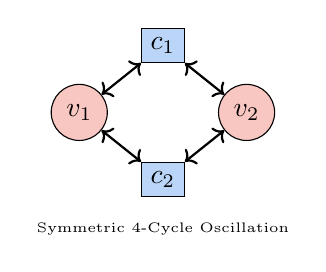
\begin{tikzpicture}[scale=0.85]
                    \node[draw, circle, fill=googlered!30] (v1) at (0, 1.5) {$v_1$};
                    \node[draw, circle, fill=googlered!30] (v2) at (2.5, 1.5) {$v_2$};
                    \node[draw, rectangle, fill=googleblue!30] (c1) at (1.25, 2.5) {$c_1$};
                    \node[draw, rectangle, fill=googleblue!30] (c2) at (1.25, 0.5) {$c_2$};
                    
                    \draw[thick, <->] (v1) -- (c1);
                    \draw[thick, <->] (v2) -- (c1);
                    \draw[thick, <->] (v1) -- (c2);
                    \draw[thick, <->] (v2) -- (c2);
                    
                    \node[below=0.2cm of c2] {\tiny Symmetric 4-Cycle Oscillation};
                \end{tikzpicture}
            \end{block}
        \end{column}
    \end{columns}
\end{frame}

\begin{frame}{Why Standard BP Struggles with Quantum Codes}
    \begin{block}{The Quantum Trapping Set Problem}
        \begin{itemize}
            \item Classical LDPC codes are designed with large girth (no short cycles).
            \item Quantum LDPC codes (due to commutativity constraints $H_X H_Z^T = 0$) inherently contain abundant short cycles (length 4 and 6).
            \item These form \textbf{symmetric trapping sets}—sub-graphs that trick BP into endless oscillation.
        \end{itemize}
    \end{block}
    
    \begin{block}{The Need for OSD and Advanced Scheduling}
        \begin{itemize}
            \item \textbf{Without Scheduling}: Parallel updates bounce messages back and forth synchronously, failing to break symmetry.
            \item \textbf{Without OSD}: BP gives up when it can't converge, leaving the syndrome uncleared (logical failure).
            \item \textbf{Solution}: We must break graph symmetry (via Stochastic Scheduling) and provide an algebraic fallback (via OSD) when heuristic BP fails.
        \end{itemize}
    \end{block}
\end{frame}

\section{Tesseract-BP Architecture \& Optimization Deep-Dive}

\begin{frame}{Tesseract-BP High-Level Data Flow}
    \centering
    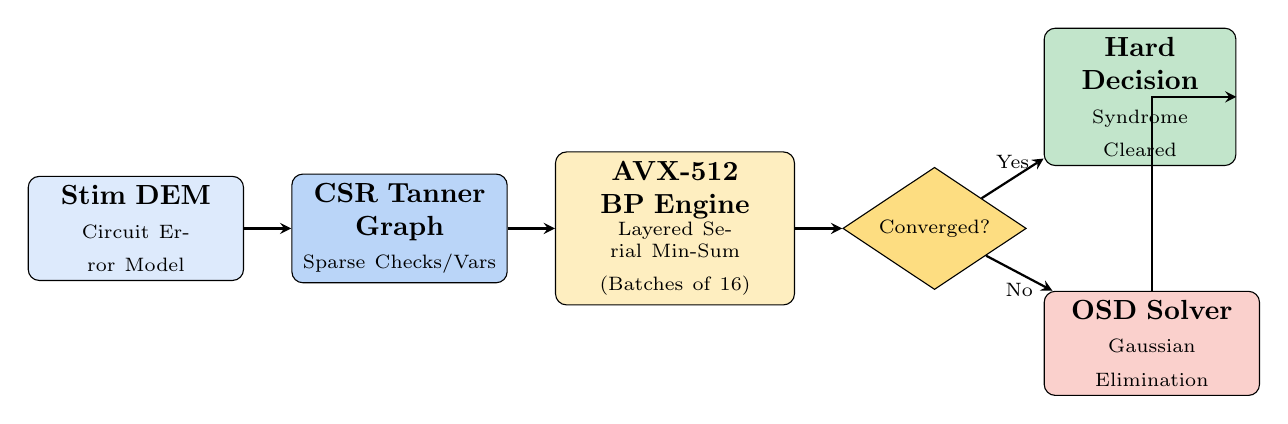
\begin{tikzpicture}[node distance=1.2cm, auto, >=stealth]
        \node [rectangle, draw, fill=googleblue!15, rounded corners, text width=2.5cm, align=center] (dem) {\textbf{Stim DEM}\\\scriptsize Circuit Error Model};
        \node [rectangle, draw, fill=googleblue!30, rounded corners, text width=2.5cm, align=center, right=0.6cm of dem] (csr) {\textbf{CSR Tanner Graph}\\\scriptsize Sparse Checks/Vars};
        \node [rectangle, draw, fill=googleyellow!25, rounded corners, text width=2.8cm, align=center, right=0.6cm of csr] (bp) {\textbf{AVX-512 BP Engine}\\\scriptsize Layered Serial Min-Sum\\(Batches of 16)};
        \node [diamond, draw, fill=googleyellow!50, align=center, right=0.6cm of bp, aspect=1.5] (check) {\scriptsize Converged?};
        \node [rectangle, draw, fill=googlegreen!30, rounded corners, text width=2.2cm, align=center, above right=0.4cm and 0.8cm of check] (out) {\textbf{Hard Decision}\\\scriptsize Syndrome Cleared};
        \node [rectangle, draw, fill=googlered!25, rounded corners, text width=2.5cm, align=center, below right=0.4cm and 0.8cm of check] (osd) {\textbf{OSD Solver}\\\scriptsize Gaussian Elimination};
        
        \draw [->, thick] (dem) -- (csr);
        \draw [->, thick] (csr) -- (bp);
        \draw [->, thick] (bp) -- (check);
        \draw [->, thick] (check) -- node[above] {\scriptsize Yes} (out);
        \draw [->, thick] (check) -- node[below] {\scriptsize No} (osd);
        \draw [->, thick] (osd) |- (out);
    \end{tikzpicture}
\end{frame}

\begin{frame}[fragile]{Architecture: Pointer-Chasing vs. Bidirectional CSR}
    \begin{columns}[T]
        \begin{column}{0.5\textwidth}
            \begin{block}{\textcolor{googlered}{Naive BP}: Pointer-Chasing Graph}
                \tiny
                \begin{lstlisting}[language=C++]
struct Node {
    std::vector<Node*> neighbors;
    std::vector<double> messages;
};
std::vector<Node*> nodes;
                \end{lstlisting}
                \normalsize
                \begin{itemize}
                    \item Follows \texttt{std::vector} memory allocations.
                    \item Nodes scattered across fragmented heap memory.
                    \item Traversing neighbors means chasing pointers $\rightarrow$ \textbf{L1/L2 Cache Miss Penalty}!
                \end{itemize}
            \end{block}
        \end{column}
        
        \begin{column}{0.5\textwidth}
            \begin{block}{\textcolor{googlegreen}{Tesseract BP}: Bidirectional CSR}
                \tiny
                \begin{lstlisting}[language=C++]
// Flat integer arrays, no pointers!
vector<int> check_to_var_indices;
vector<int> check_to_var_offsets;
vector<int> var_to_check_indices;
vector<int> var_to_check_offsets;
                \end{lstlisting}
                \normalsize
                \begin{itemize}
                    \item \textbf{Compressed Sparse Row (CSR)}: Graph represented as 1D contiguous arrays.
                    \item \textbf{Bidirectional}: Fast $O(1)$ neighborhood lookups in both directions ($C \rightarrow V$ and $V \rightarrow C$).
                    \item Sequential memory access ensures hardware prefetcher efficiency.
                \end{itemize}
            \end{block}
        \end{column}
    \end{columns}
\end{frame}

\begin{frame}[fragile]{Optimization 1: Memory Foundation Rewrite (Interleaved 1D Array)}
    \begin{columns}[T]
        \begin{column}{0.5\textwidth}
            \begin{block}{\textcolor{googlered}{BEFORE}: Vector of Vectors (Non-Interleaved)}
                \tiny
                \begin{verbatim}
Shot 0:  [ Var0, Var1, Var2, ..., VarN ]
Shot 1:  [ Var0, Var1, Var2, ..., VarN ]  (RAM Gap)
Shot 2:  [ Var0, Var1, Var2, ..., VarN ]  (RAM Gap)
...
Shot 15: [ Var0, Var1, Var2, ..., VarN ]
                \end{verbatim}
                \normalsize
                \begin{itemize}
                    \item Loading Variable $V_i$ across 16 SIMD shots required fetching \textbf{16 separate RAM addresses}.
                    \item Transfers 1,024 bytes to extract 64 bytes of data $\rightarrow$ \textbf{L1 Cache Flushed!}
                \end{itemize}
            \end{block}
        \end{column}
        
        \begin{column}{0.5\textwidth}
            \begin{block}{\textcolor{googlegreen}{AFTER}: Flat Interleaved 1D Array}
                \tiny
                \begin{verbatim}
RAM: [ Var0_S0..S15 | Var1_S0..S15 | Var2_S0..S15 ]
                \end{verbatim}
                \normalsize
                \begin{itemize}
                    \item Memory address: \texttt{posteriors\_flat[v * 16 + b]}.
                    \item All 16 shot streams for Variable $V_i$ sit \textbf{physically contiguous} in RAM (64 bytes).
                    \item \textbf{1 SIMD Aligned Load} = 1 L1 Cache Line Hit!
                \end{itemize}
            \end{block}
        \end{column}
    \end{columns}
\end{frame}

\begin{frame}{Optimization 2: Horizontal Layered Serial Scheduling}
    \begin{block}{Algorithmic Transformation}
        Instead of updating variable node posteriors sequentially, iteration loops operate directly over \textbf{check nodes ($c \in C$)}:
        \begin{enumerate}
            \item For each check node $c$, calculate check-to-variable updates dynamically:
                  $$Q_{c,v} = L_v - R_{c,v}$$
            \item Compute the updated check message $R'_{c,v}$ using Min-Sum across check neighbors.
            \item Immediately update the variable posteriors in RAM:
                  $$L'_v = Q_{c,v} + R'_{c,v}$$
        \end{enumerate}
    \end{block}
    
    \begin{block}{50\% Memory Bandwidth Reduction}
        \begin{itemize}
            \item By performing $L_v - R_{c,v}$ on the fly, the explicit 2D message matrix $R_{c,v}$ is \textbf{completely eliminated from memory}!
            \item Reduces BP memory payload by \textbf{50\%}, doubling memory bus efficiency.
        \end{itemize}
    \end{block}
\end{frame}

\begin{frame}{Optimization 3: Explicit AVX-512 SIMD Vectorization}
    \begin{block}{Vector Register Mapping}
        16 parallel decoding shots ($32$-bit integer LLRs) map directly into one 512-bit AVX-512 register (\texttt{\_\_m512i}):
        $$16 \times 32 \text{ bits} = 512 \text{ bits}$$
    \end{block}
    
    \begin{block}{Core AVX-512 Intrinsic Operations}
        \begin{itemize}
            \item \texttt{\_mm512\_abs\_epi32}: Compute absolute LLR magnitudes for 16 shots simultaneously.
            \item \texttt{\_mm512\_min\_epi32}: Track minimum LLRs (\texttt{min1}, \texttt{min2}) without conditional branching latency.
            \item \texttt{\_mm512\_sub\_epi32} / \texttt{\_mm512\_add\_epi32}: Vectorized posterior updates.
            \item \texttt{\_mm512\_mask\_blend\_epi32} / \texttt{\_mm512\_movepi32\_mask}: Masked updates for active unconverged shots.
        \end{itemize}
    \end{block}
\end{frame}

\begin{frame}[fragile]{Optimization 4: Stochastic Check-Node Schedule Permutations}
    \begin{columns}[T]
        \begin{column}{0.55\textwidth}
            \begin{block}{Breaking Trapping Sets with PRNG}
                \begin{itemize}
                    \item Fixed schedule $0 \rightarrow M-1$ locks into symmetric LDPC trapping sets.
                    \item \textbf{Solution}: Apply Fisher-Yates check-node permutation before each BP iteration using a fast \textbf{Xorshift64 PRNG}.
                    \item Because memory is interleaved in 64-byte blocks, random check node hopping incurs \textbf{zero SIMD alignment penalty}!
                    \item Resolves trapping sets in Color Codes and Bivariate Bicycle codes seamlessly.
                \end{itemize}
            \end{block}
        \end{column}
        
        \begin{column}{0.42\textwidth}
            \begin{block}{Xorshift64 PRNG}
                \scriptsize
                \begin{lstlisting}[language=C++]
inline uint64_t xorshift64(uint64_t &state) {
    uint64_t x = state;
    x ^= x << 13;
    x ^= x >> 7;
    x ^= x << 17;
    return state = x;
}
                \end{lstlisting}
            \end{block}
        \end{column}
    \end{columns}
\end{frame}

\begin{frame}{Optimization 5: Ordered Statistic Decoding (OSD) Integration}
    \begin{block}{Algebraic Fallback Pipeline}
        When BP fails to clear all syndrome bits after \texttt{max\_iter}:
        \begin{enumerate}
            \item \textbf{Reliability Ordering}: Sort variable nodes by absolute LLR magnitude $|L_v|$ (highest magnitude = highest reliability).
            \item \textbf{Information Set Basis}: Perform column-pivoted Gaussian elimination on $H$ matrix over SIMD bitsets (\texttt{stim::simd\_bits}).
            \item \textbf{Perturbation Search}:
                  \begin{itemize}
                      \item \textbf{OSD-0}: Hard decision on basis + solver solution.
                      \item \textbf{OSD-1}: Test 1-bit perturbations on least reliable columns.
                      \item \textbf{OSD-2}: Test 2-bit perturbations on candidate combinations.
                  \end{itemize}
            \item Select candidate matching syndrome $s$ with minimum total weight/cost.
        \end{enumerate}
    \end{block}
\end{frame}

\section{Benchmarks, Empirical Results \& Future Outlook}

\begin{frame}{Benchmark Methodology \& Environment}
    \begin{block}{Evaluation Setup}
        \begin{itemize}
            \item \textbf{Hardware}: 48-vCPU Intel Xeon Workstation with AVX-512 vector support.
            \item \textbf{Sample Size}: 100,000 Monte Carlo shots per quantum code configuration.
            \item \textbf{Code Benchmark Families}:
                  \begin{itemize}
                      \item Surface Codes ($d=3, 5, 7, 9$, physical error rate $p=0.001$).
                      \item Color Codes ($d=5, 7$ Superdense).
                      \item Bivariate Bicycle Codes ($[[72,12,6]]$, $[[90,8,10]]$, $[[108,8,10]]$, $[[144,12,12]]$).
                  \end{itemize}
        \end{itemize}
    \end{block}
\end{frame}

\begin{frame}{Empirical Benchmark Throughput Comparison}
    \centering
    \scriptsize
    \begin{tabular}{l l r r c}
        \toprule
        \textbf{Quantum Code Family} & \textbf{Decoder Config} & \textbf{Baseline (shots/s)} & \textbf{Optimized (shots/s)} & \textbf{Speedup} \\
        \midrule
        \textbf{Surface Code ($d=3$, $p=0.001$)} & `serial-batched` (BP) & 306,867.6 & \textbf{922,330.5} & \textbf{3.01x (+200.6\%)} \\
        \textbf{Surface Code ($d=5$, $p=0.001$)} & `serial-batched` (BP) & 30,728.0 & \textbf{161,361.1} & \textbf{5.25x (+425.1\%)} \\
        \textbf{Surface Code ($d=7$, $p=0.001$)} & `serial-batched` (BP) & 6,777.6 & \textbf{32,631.1} & \textbf{4.81x (+381.5\%)} \\
        \textbf{Surface Code ($d=9$, $p=0.001$)} & `serial-batched` (BP) & 2,258.9 & \textbf{8,660.9} & \textbf{3.83x (+283.4\%)} \\
        \midrule
        \textbf{Color Code Superdense ($d=5$)} & `serial-batched` (BP) & 14,815.3 & \textbf{65,647.4} & \textbf{4.43x (+343.1\%)} \\
        \textbf{Color Code Superdense ($d=7$)} & `serial-batched` (BP) & 3,062.9 & \textbf{9,399.2} & \textbf{3.07x (+206.9\%)} \\
        \midrule
        \textbf{Bivariate Bicycle $[[72,12,6]]$} & `serial-batched + OSD-0` & 1,384.9 & \textbf{4,142.6} & \textbf{2.99x (+199.1\%)} \\
        \textbf{Bivariate Bicycle $[[72,12,6]]$} & `serial-batched + OSD-1` & 978.5 & \textbf{2,165.6} & \textbf{2.21x (+121.3\%)} \\
        \textbf{Bivariate Bicycle $[[90,8,10]]$} & `serial-batched + OSD-0` & 539.3 & \textbf{1,466.1} & \textbf{2.72x (+171.8\%)} \\
        \textbf{Bivariate Bicycle $[[108,8,10]]$} & `serial-batched + OSD-0` & 414.3 & \textbf{1,096.1} & \textbf{2.65x (+164.6\%)} \\
        \textbf{Bivariate Bicycle $[[144,12,12]]$} & `serial-batched + OSD-0` & 208.9 & \textbf{462.0} & \textbf{2.21x (+121.2\%)} \\
        \bottomrule
    \end{tabular}
\end{frame}

\begin{frame}{Performance Analysis \& Speedup Drivers}
    \begin{columns}[T]
        \begin{column}{0.48\textwidth}
            \begin{block}{Why Did Throughput Increase 2.2x to 5.25x?}
                \begin{itemize}
                    \item \textbf{L1 Cache locality}: 1D Interleaved layout eliminated L1 cache flushes during SIMD loads.
                    \item \textbf{50\% Bandwidth Reduction}: Eliminating $R_{c,v}$ 2D message tables doubled memory bus efficiency.
                    \item \textbf{AVX-512 Intrinsics}: 16-shot SIMD vector registers executed without branch latency.
                \end{itemize}
            \end{block}
        \end{column}
        
        \begin{column}{0.48\textwidth}
            \begin{block}{Trapping Set Resolution}
                \begin{itemize}
                    \item Stochastic check node permutations broke static trapping set loops in Bivariate Bicycle and Color codes.
                    \item Average iterations to convergence dropped significantly across complex qLDPC topologies!
                \end{itemize}
            \end{block}
        \end{column}
    \end{columns}
\end{frame}

\begin{frame}{Future Roadmap \& Open Scope}
    \begin{block}{Next Steps for Tesseract-BP}
        \begin{enumerate}
            \item \textbf{Vectorized OSD Gaussian Elimination}: Batching column-pivoted Gaussian elimination over 16-shot SIMD blocks when BP fails to converge.
            \item \textbf{OSD-2 Priority Search Pruning}: Restricting perturbation search space candidates using LLR priority bounds.
            \item \textbf{BP-Guided Search Integration}: Feeding BP posteriors directly into Tesseract A* Search heuristic cost matrices ($g(n) + h(n)$).
        \end{enumerate}
    \end{block}
\end{frame}


% --- Closing Slide ---
\begin{frame}{Summary \& Q\&A}
    \begin{block}{Key Takeaways}
        \begin{itemize}
            \item \textbf{Tesseract Decoding Vision}: Tiered QEC workflow (BP $\rightarrow$ MultiPass $\rightarrow$ Full Tesseract Search).
            \item \textbf{High-Throughput BP Engine}: 1D Interleaved Flat Array + Horizontal Layered Serial Min-Sum.
            \item \textbf{AVX-512 Vectorization}: 16 parallel shot streams processed in a single 512-bit register.
            \item \textbf{LDPC Trapping Set Solution}: Stochastic Fisher-Yates schedule permutations.
            \item \textbf{Empirical Gains}: \textbf{2.2x to 5.25x throughput speedup} across Surface, Color, and Bivariate Bicycle codes.
        \end{itemize}
    \end{block}
    \centerline{\Huge\textcolor{googleblue}{\textbf{Questions \& Discussion}}}
\end{frame}

\end{document}
